% UNO Flip Remix - Software Requirements Specification
\documentclass[12pt]{article}
\usepackage{xcolor}
\usepackage[normalem]{ulem} % for strikethrough
\usepackage{geometry}
\usepackage{hyperref}
\geometry{margin=1in}
\usepackage{array}
\usepackage{graphicx}
\usepackage{float}
\usepackage{longtable}
\usepackage{tabularx}

% Red strikethrough command
\newcommand{\removed}[1]{\textcolor{red}{\sout{#1}}}
% Green addition command
\newcommand{\added}[1]{\textcolor{green}{#1}}


\title{Software Requirements Specification for UNO Flip}
\author{Team 24 \\ Mingyang Xu \\ Kevin Ishak \\ Zain-Alabedeen Garada \\ Jianhao Wei \\ \removed{Andy Liang}}
\date{April 2, 2025}

\begin{document}

\maketitle

\tableofcontents

\section{Purpose of the Document}

\subsection{Introduction}
This document is meant to specify the high-level software requirements in the early stages of the development of our project. This includes the stakeholders, constraints, scope, functional requirements, and non-functional requirements of our project. The information in this document serves as the basis for the later stages of our software development process and maybe subject to modification as the project continues.

\subsection{Intended Reader}
The intended reader of this document includes:
\begin{itemize}
    \item \textbf{Ourselves} for future references
    \item \textbf{Clients} for evaluating the academic and technical criteria
    \item \textbf{Stakeholders} for understanding the purpose of the project and determine how their contribution can be integrated
    \item \textbf{Supervisors} for supervise the project and give critical feedback.
\end{itemize}

\section{Purpose of the Project}

\subsection{User Business}
The UNO Flip Remix project is designed to bring the classic UNO Flip card game into the digital gaming landscape, catering to the growing demand for online and interactive multiplayer experiences. By targeting casual gamers, students, and board game enthusiasts, the project aims to replicate the traditional game's excitement while incorporating modern features such as AI opponents and real-time synchronization. As part of a capstone initiative, the project not only provides an engaging product for the market but also serves an educational purpose, allowing the development team to apply software engineering principles and tackle real-world challenges.

\subsection{Goals of the Project}
The UNO Flip Remix project is part of a capstone design initiative undertaken by Team 24. The objective of this project is to develop a multiplayer card game based on the popular UNO Flip game, integrating real-time synchronization and basic AI functionalities to simulate player interactions. \removed{The project will focus on both front-end and back-end development to ensure a seamless user experience, using a combination of JavaScript for core functionalities and TensorFlow for reinforcement learning to implement AI behaviors.} \added{The game will be developed entirely in C\# using the Unity engine, with all game logic, AI behavior, and user interface handled within the Unity framework. AI functionality will be implemented using rule-based logic rather than machine learning.}

\section{Mandated Constraints}

\subsection{Solution Constraints}
\removed{The UNO Flip Remix project is constrained by the technologies chosen for development, including JavaScript and Node.js for both front-end and back-end implementations. Socket.IO will be used to manage real-time communication for multiplayer gameplay, while TensorFlow is employed for integrating AI functionalities. These technologies set limitations on how the system can be built, as they must work together seamlessly to ensure cross-platform compatibility and efficient performance.}
\added{The UNO Flip Remix project is constrained by the use of the Unity engine and the C\# programming language. All gameplay mechanics, animations, and AI logic will be implemented within the Unity framework. Unity’s built-in networking systems or compatible multiplayer frameworks will handle real-time synchronization.}
Additionally, all code must adhere to standard best practices for modularity and maintainability.

\subsection{Implementation Environment of the Current System}
\removed{The game is designed to operate as a web-based application, running on various web browsers such as Chrome, Firefox, Safari, and Edge. The development environment utilizes a combination of JavaScript for the client-side, Node.js for the server-side, and Socket.IO for managing real-time data synchronization. The implementation environment does not include support for mobile apps or offline gameplay in the initial phase, though the system is designed with potential future expansion to mobile platforms in mind.}
\added{The game is designed to operate as a standalone application built with Unity, targeting desktop platforms such as Windows and macOS. The initial implementation will not support mobile or browser-based gameplay, though expansion to other platforms may be considered in future versions. Unity’s development environment and build pipeline will be used throughout the implementation process.}

\subsection{Off-the-Shelf Software}
\removed{The project will use off-the-shelf software components such as TensorFlow for AI capabilities and Socket.IO for real-time communication. Additionally, standard libraries for web development (e.g., React or Express.js) may be used to accelerate development. These off-the-shelf components will be integrated into the custom codebase to provide essential functionality like AI decision-making and low-latency multiplayer synchronization.}
\added{The project will use Unity as the primary development platform and may include Unity Asset Store packages to assist with features like UI design, animation handling, or multiplayer support. Unity’s built-in systems for physics, animation, and networking will form the foundation for game functionality.}

\subsection{Other Stakeholders}
\removed{Other stakeholders include the development team (Team 24), system administrators, and potential future contributors. The development team is responsible for the end-to-end creation of the game, including coding, testing, and delivering the final product. System administrators will manage the server-side operations, addressing any technical issues to ensure smooth performance and availability. Future developers or contributors, such as open-source enthusiasts, may also be involved in extending the game’s features, enhancing AI, or scaling the system.}
\added{Other stakeholders include system administrators and potential future contributors. System administrators will manage infrastructure deployment, monitor performance, and apply updates to ensure system reliability. Future contributors, such as developers in academic or industry settings, may support game improvements or create additional content. The development team is not considered a stakeholder in the traditional sense, as their responsibilities are already documented elsewhere in the project and do not qualify as a separate stakeholder group.}

\subsection{Hands-On Users of the Project}
\removed{Hands-on users consist of the players who will interact with the game, system administrators who ensure that the game servers run efficiently, and developers involved in both the initial development and any future maintenance. Players will experience the game's features firsthand, providing valuable feedback on usability and gameplay mechanics, while administrators will handle technical aspects like server maintenance and troubleshooting.}
\added{Hands-on users include players who interact directly with the game, experiencing its gameplay and visuals, and providing feedback on user interface and mechanics. System administrators are also hands-on users responsible for maintaining backend services, applying updates, and resolving technical issues.}

\subsection{Personas}
\removed{The main personas for this project include casual gamers and game enthusiasts who enjoy traditional card games in a digital format with creative element. These personas help guide design choices to cater to different user expectations, such as the ease of use for players and overcome the physical limitations presented in the physical card games.}
\added{The primary personas are:
\begin{itemize}
    \item \textbf{Casual Gamers:} Seek quick, intuitive gameplay with minimal onboarding. Prefer straightforward controls, simple visuals, and quick matchmaking.
    \item \textbf{Game Enthusiasts:} Appreciate deeper strategy, polished graphics (especially 3D rendering), customization options, and performance metrics.
\end{itemize}
These personas guide the design of both gameplay mechanics and UI/UX considerations. Requirements in later sections will be refined to reflect how the system supports each group.}

\subsection{Priorities Assigned to Users}
\removed{High priority is assigned to casual gamers and game enthusiasts who are expected to form the largest user base. Medium priority is assigned to game critics or potential future developers who could contribute to the project’s open-source aspects or further development.}
\added{High priority is given to casual gamers and game enthusiasts, as they represent the primary users and are directly affected by usability, performance, and visual appeal. Medium priority is assigned to future contributors, such as developers who may expand the project after its initial release. Low priority is given to game critics, as their feedback, while valuable, is not central to the iterative development process.}

\subsection{User Participation}
\removed{Players will provide feedback through gameplay experiences, which will be used for future improvements. Users will participate in the development process by providing feedback during alpha and beta testing phases. Their input on gameplay, user interface, and any encountered issues will help shape the final product and guide future iterations. Players’ suggestions may influence the addition of new features, refinement of existing mechanics, or improvements in AI behavior.}
\added{Players will provide feedback during structured alpha and beta testing periods through in-game prompts or optional surveys. This feedback will be reviewed and categorized to guide future iterations. As this project no longer includes adaptive AI behavior, feedback will focus on gameplay balancing, rule clarity, 3D visual comfort (e.g., accessibility for those with motion sensitivity), and responsiveness of controls.}

\subsection{Maintenance Users and Service Technicians}
\removed{System administrators will perform maintenance tasks such as server monitoring, software updates, and troubleshooting technical issues to ensure uninterrupted gameplay. Service technicians may also assist with more complex issues involving server configuration or scaling, particularly when the user base increases or when adding new features requires infrastructure changes.}
\added{System administrators will perform platform maintenance such as patch deployments, configuration of game servers (e.g., Unity game instance hosting), and log monitoring. While the game is primarily deployed for academic purposes, service technicians may assist in setting up or debugging build pipelines and platform compatibility for lab demonstrations or future reuse.}

\section{Mandated Constraints}

\subsection{Solution Constraints}
\removed{The UNO Flip Remix project is constrained by the technologies chosen for development, including JavaScript and Node.js for both front-end and back-end implementations. Socket.IO will be used to manage real-time communication for multiplayer gameplay, while TensorFlow is employed for integrating AI functionalities. These technologies set limitations on how the system can be built, as they must work together seamlessly to ensure cross-platform compatibility and efficient performance.} \added{The UNO Flip Remix project is developed using C\# in Unity, which introduces specific constraints tied to that platform. Unity dictates how real-time interactions, animations, multiplayer architecture, and 3D rendering are structured. All code must follow Unity’s framework guidelines and ensure performance efficiency on supported platforms.} Additionally, all code must adhere to standard best practices for modularity and maintainability.

\subsection{Implementation Environment of the Current System}
\removed{The game is designed to operate as a web-based application, running on various web browsers such as Chrome, Firefox, Safari, and Edge. The development environment utilizes a combination of JavaScript for the client-side, Node.js for the server-side, and Socket.IO for managing real-time data synchronization. The implementation environment does not include support for mobile apps or offline gameplay in the initial phase, though the system is designed with potential future expansion to mobile platforms in mind.} \added{The game is developed in Unity and will operate as a standalone desktop application, initially for Windows systems. The implementation environment leverages Unity’s rendering engine for 3D graphics and C\# scripting. Multiplayer synchronization is built using Unity’s networking stack. The system is not designed for mobile or web-based play in the initial version but may support cross-platform builds in the future.}

\subsection{Partner or Collaborative Applications}
There are no partner or collaborative applications required for the initial release of the UNO Flip Remix game.

\subsection{Off-the-Shelf Software}
\removed{The project will use off-the-shelf software components such as TensorFlow for AI capabilities and Socket.IO for real-time communication. Additionally, standard libraries for web development (e.g., React or Express.js) may be used to accelerate development. These off-the-shelf components will be integrated into the custom codebase to provide essential functionality like AI decision-making and low-latency multiplayer synchronization.} \added{The project uses Unity as the core development platform and C\# for scripting. Unity provides many off-the-shelf packages and components for handling animation, 3D rendering, audio playback, and physics. For multiplayer capabilities, Unity’s built-in Netcode (or compatible networking frameworks such as Mirror or Photon Fusion) will be used.}

\subsection{Anticipated Workplace Environment}
\removed{The UNO Flip Remix game is intended to be played on standard desktop and laptop computers, using modern web browsers. Players are expected to access the game through stable internet connections, as multiplayer synchronization requires continuous online connectivity.} \added{The UNO Flip Remix game is intended to be played on desktop computers running Windows OS. A stable internet connection is required to enable multiplayer sessions. The system should be run on machines capable of rendering 3D content with sufficient frame rates, using mid-range or higher GPUs. This ensures the game runs smoothly and without performance issues caused by hardware limitations.}

\subsection{Schedule Constraints}
The project follows a Scrum development process with weekly sprints, which dictates the pace and structure of the project. The capstone project's academic timeline also constrains the schedule, requiring the game to be completed by a predetermined deadline for evaluation.

\subsection{Budget Constraints}
The project is constrained by a limited budget provided by the Capstone course, which covers essential development tools and technologies.

\subsection{Enterprise Constraints}
The development of the UNO Flip Remix game must comply with McMaster University project guidelines and meet academic criteria. In addition, adherence to open-source standards where applicable is required to allow future community involvement.

\section{Naming Conventions and Terminology}

\subsection{Glossary of All Terms, Including Acronyms, Used by Stakeholders Involved in the Project}

\begin{itemize}
    \item \textbf{UNO} – A card game with specific rules and card actions.
    \item \textbf{AI} – Artificial Intelligence. \added{- Used for non-player rule-based decision-making.}
    \item \removed{ \textbf{ML} – Machine Learning.}
    \item \removed{\textbf{RL} – Reinforcement Learning.}
    \item \removed{\textbf{3D Rendering} – Three-dimensional graphics rendering system.}
    \item \added{\textbf{2D Rendering} - The process of drawing and animating two-dimensional assets on the screen. The game will be entirely 2D, using 2D sprites and effects.}
    \item \removed{ \textbf{NPC} – Non-Player Character. }
    \item \removed{ \textbf{CI/CD} – Continuous Integration / Continuous Deployment. }
    \item \textbf{DLC} – Downloadable Content.
    \item \textbf{GDPR} – General Data 
    Protection Regulation.
    \item \added{\textbf{UI} – User Interface. Refers to all the visual and interactive components players use to interact with the game (e.g., menus, buttons, card visuals).}
    \item \added{\textbf{UX} – User Experience. Encompasses the overall player experience including ease of use, accessibility, and immersion.}
\end{itemize}

\section{Relevant Facts and Assumptions}

\subsection{Relevant Facts}
\removed{The project is based on the popular UNO Flip card game, which has well-established gameplay mechanics. JavaScript and Node.js are being used as the primary languages for front-end and back-end development, ensuring cross-platform compatibility. Socket.IO is employed to handle real-time communication, enabling multiplayer gameplay with low-latency synchronization. TensorFlow is used for the AI implementation, which will control non-player characters (NPCs) during the game.}
\added{The UNO Flip Remix project is being developed using the Unity engine with C\# scripting and follows a 2D design approach. Multiplayer functionality is implemented using Unity’s networking features, and the AI is rule-based rather than learning-based.}

\begin{itemize}
    \item \textbf{Game Origin:} The project is based on the popular UNO Flip card game, which has well-established gameplay mechanics.
    \item \textbf{Technology Stack:} \removed{JavaScript and Node.js are being used as the primary languages for front-end and back-end development, ensuring cross-platform compatibility. Socket.IO is employed to handle real-time communication, enabling multiplayer gameplay with low-latency synchronization. TensorFlow is used for the AI implementation, which will control non-player characters (NPCs) during the game.}
    \added{The project is being implemented in C\# using the Unity engine. Multiplayer capabilities are enabled through Unity's networking libraries, and AI behavior is driven by rule-based logic designed to mimic basic strategic play.}
    \item \textbf{Cross-Platform Support:} \added{Unity provides compatibility for cross-platform builds, though the initial release will target Windows.}
\end{itemize}

\subsection{Business Rules}
\begin{itemize}
    \item \textbf{Game Integrity:} The rules of UNO Flip must be strictly followed. The system will enforce game logic, including player turns, card actions, and the application of special card effects like "Flip," "Skip," or "Draw." \added{These rules are also reflected in Functional Requirements TMR1, EGHR1, and GSR1.}
    \item \textbf{Player Limits:} The game will allow a minimum of 2 players and a maximum of 4 players in multiplayer mode. Additional player capacities could be explored in future updates.
    \item \textbf{Card Distribution:} Each player will receive 7 cards at the start of the game. The system will randomize the deck to ensure fairness in card distribution.
    \item \textbf{Game Modes:} Only the "standard" and "flip" sides of the game will be available in the initial version. Future iterations may add variations to the gameplay or more modes.
    \item \textbf{No Cheating Policy:} Any attempts to manipulate or cheat the system (e.g., unauthorized access to player card data) will result in immediate disqualification from the match and possibly a temporary or permanent account ban.
    \item \textbf{Matchmaking:} Players will be automatically matched with opponents based on skill levels or allowed to invite friends to private games.
\end{itemize}

\subsection{Assumptions}
\begin{itemize}
    \item Players are expected to have reliable internet connections, ensuring smooth gameplay and minimal latency issues. \added{This assumption supports Requirements MSR1 and MSR2.}
    \item Players will use modern browsers (e.g., Chrome, Firefox) \removed{that support JavaScript and WebSockets} \added{that are compatible with Unity WebGL builds}.
    \item \removed{The AI will initially be rule-based, with the potential to evolve into more complex AI using machine learning techniques in future iterations.}
    \item \added{The AI will use rule-based decision-making only. There are no plans to use machine learning. This supports FR TMR1 and UC-04 (AI Turn).}
    \item The game will initially support up to 4 players, with scalability planned for future updates. \added{(Related to Requirement GSR1)}
    \item Players have a basic understanding of the rules of UNO Flip. Tutorials will be available for new users but not mandatory for experienced players. \added{(Linked to Usability Requirement LR1)}
\end{itemize}

\section{The Scope of the Work}

\subsection{The Current Situation}
Currently, UNO Flip is a popular physical card game enjoyed by small groups of players. Players must be physically present to engage in gameplay, shuffling decks, and manually handling game mechanics like drawing cards and flipping the deck. The game lacks a \added{smooth and enjoyable}. Additionally, tracking scores and enforcing rules is dependent on the players themselves, which may lead to errors or misunderstandings.

\subsection{The Context of the Work}
The project aims to develop an online, multiplayer version of UNO Flip that not only mimics the physical game but also enhances the user experience with engaging and dynamic features. This digital version will allow players to connect and play in real-time, regardless of location, and will automatically enforce all game rules to ensure fairness. \removed{Visually stunning animations and dynamic features will further enhance the excitement, especially during special moves such as “Flip,” “Draw,” and “Reverse,” making the game more immersive and enjoyable.} \added{Animations and visual feedback will enhance the excitement, especially during special moves such as “Flip,” “Draw,” and “Reverse,” making the game more responsive and enjoyable.}

\subsection{Work Partitioning}

\textbf{Front-End:} The front-end development includes all \added{UI and UX tasks}, such as designing a \removed{visually engaging} \added{user friendly} game interface, implementing animations for card actions, \removed{and ensuring responsiveness across devices (e.g., desktops, tablets, mobile).} \added{and ensuring smooth interaction and responsiveness on desktop and laptop computers.} Front-end developers will also handle real-time interactions, including drag-and-drop functionality for card movements, interactive menus, and chat integration for multiplayer communication.

\textbf{Back-End:} The back-end development will focus on building and maintaining the server-side infrastructure. This includes implementing game logic, managing player connections, handling real-time synchronization of game states, user authentication, matchmaking, and turn-based systems. \removed{Node.js and WebSockets will be used for real-time communication, while AI logic will be implemented for single-player or AI-assisted multiplayer games.} \added{The back-end development consists of a Unity-based TCP server solution that manages game logic, session state, and player interactions. This includes turn management, AI behavior logic, and client-server communication over TCP. The server ensures that all actions are synchronized properly across connected clients.}

\subsection{Specifying a Business Use Case (BUC)}

\textbf{Player Login:} Players must log into the platform using a unique ID or credentials. Upon logging in, the system retrieves the player's profile, game history, and scores. The system ensures the player's session is secure and maintains continuity between different gaming sessions. \added{This login process is a prerequisite for Requirement AR1.} \\

\textbf{Game Setup:} Once logged in, players can create a game room or join an existing room. The game setup includes customizable options like the number of players, game mode (e.g., standard or flip mode), and AI opponents. The host of the game room has administrative rights to set and adjust these configurations. \added{This is linked to Functional Requirement GSR1.} \\

\textbf{Turn Management:} The system automatically manages turn-taking during the game, enforcing the rules to ensure that each player performs valid moves. The system also ensures the correct order of play is followed and handles the transition between players smoothly. \added{This supports Requirement TMR1.} \\

\textbf{AI Opponents:} The AI players will follow predefined strategies, making decisions in real-time. \removed{The AI’s behavior will initially be rule-based, with future potential for more advanced strategies using machine learning techniques.} \added{The AI’s behavior will be strictly rule-based and deterministic.} \added{This supports Use Case UC-04 and Requirement AI1.} \\

\textbf{Scoring:} At the end of each game, the system calculates scores based on the cards remaining in each player's hand. These scores will be stored in the player's profile, and a leaderboard will track the highest scores. Additionally, player statistics, such as the number of games played and win/loss ratio, will be updated after each game. \added{This aligns with Requirement SSR1.}

\section{Business Data Model and Data Dictionary}

\subsection{Business Data Model}
The following entities and attributes represent the core of the game’s business data model:

\begin{itemize}
    \item \textbf{Player:}
    \begin{itemize}
        \item \removed{\textbf{PlayerID:} Unique identifier for the player.}
        \item \removed{\textbf{Username:} The name displayed during the game.}
        \item \removed{\textbf{Wins:} Total number of games won.}
        \item \removed{\textbf{Losses:} Total number of games lost.}
        \item \removed{\textbf{CurrentHand:} A list of cards the player holds.}
        \item \added{\textbf{playerName:} The display name of the player shown in-game.}
        \item \added{\textbf{playerHand:} The list of cards currently held by the player.}
        \item \added{\textbf{IsHuman:} Boolean flag indicating whether the player is human or AI-controlled.}
        \item \added{\textbf{playerHandTransform:} Reference to the UI transform used to display the human player's hand.}
        \item \added{\textbf{aiHandTransform:} References to the UI transforms used to display AI players' hands.}
        \item \added{\textbf{startingHandSize:} Number of cards each player starts with at the beginning of a match.}
    \end{itemize}

    \item \textbf{Game:}
    \begin{itemize}
        \item \textbf{GameID:} Unique identifier for each game session.
        \item \removed{\textbf{GameState:} The current state of the game (e.g., "In Progress," "Completed").}
        \item \removed{\textbf{TurnOrder:} The order of players in the game.}
        \item \removed{\textbf{CurrentDeck:} A shuffled list of cards.}
        \item \removed{\textbf{DiscardPile:} The cards that have been played and discarded.}
        \item \added{\textbf{players:} A list of \texttt{Player} objects participating in the game.}
        \item \added{\textbf{deck:} The deck of cards used during gameplay.}
        \item \added{\textbf{numberOfAiPlayers:} Integer indicating the number of AI players.}
        \item \added{\textbf{startingHandSize:} Integer indicating how many cards each player starts with.}
        \item \added{\textbf{currentPlayer:} Index of the player whose turn it currently is.}
        \item \added{\textbf{playDirection:} Integer indicating play direction: \texttt{1} for clockwise, \texttt{-1} for counterclockwise.}
        \item \added{\textbf{discardPileTransform:} Reference to the visual location where played cards are stacked.}
        \item \added{\textbf{topCard:} Reference to the last played card (CardDisplay).}
        \item \added{\textbf{topColour:} The current active colour declared by a wild card.}
        \item \added{\textbf{unoCalled:} Boolean flag to indicate if a player has called UNO.}
        \item \added{\textbf{wildPanel:} UI element allowing the player to choose a colour for wild cards.}
        \item \added{\textbf{winPanel:} UI panel shown at the end of the game.}
        \item \added{\textbf{winningText:} Text displaying the winning player.}
        \item \added{\textbf{playerHighlights:} List of UI images used to indicate which player's turn it is.}
        \item \added{\textbf{playerCardCount:} List of UI elements showing how many cards each player has.}
        \item \added{\textbf{messageText:} Text element displaying system messages.}
        \item \added{\textbf{humanHasTurn:} Boolean that identifies whether the human player has control of the current turn.}
    \end{itemize}

    \item \textbf{Card:}
    \begin{itemize}
        \item \textbf{CardID:} Unique identifier for the card.
        \item \textbf{Color:} The color of the card (e.g., red, yellow, green, blue).
        \item \textbf{Value:} The value of the card (e.g., 1-9, Draw 2, Skip, Reverse, Flip, Wild).
        \item \added{\textbf{IsFlipped:} Boolean, indicates whether the card is showing its flipped side.}
        \item \added{\textbf{CardFront:} The visible side of the card, containing value and color.}
        \item \added{\textbf{CardBack:} The flipped side of the card, with alternate value and color.}
        \item \added{\textbf{CardState:} Enum, either FRONT or BACK, indicating which side is active.}
        \item \added{\textbf{IsPlayable:} Boolean flag checked during interactions to validate if the card can be played.}
    \end{itemize}

    \item \textbf{Deck:}
    \begin{itemize}
        \item \textbf{DeckID:} Unique identifier for each deck.
        \item \textbf{Cards:} List of all cards in the deck, including both standard and flipped sides.
        \item \added{\textbf{Draw():} Method that removes and returns the top card from the deck.}
        \item \added{\textbf{Shuffle():} Method that randomizes the order of cards in the deck at the start of each game.}
        \item \added{\textbf{InitializeDeck():} Method called by the GameManager to build the deck with all necessary cards.}
    \end{itemize}

    \item \added{\textbf{WildCardSelection:}
    \begin{itemize}
        \item \textbf{SelectedWildColor:} Represents the player's selected color after playing a Wild or Wild Draw card.
    \end{itemize}}

    \item \added{\textbf{TurnState:}
    \begin{itemize}
        \item \textbf{CurrentPlayerIndex:} Index of the player whose turn it is.
        \item \textbf{PlayDirection:} Indicates direction of play (1 for clockwise, -1 for counterclockwise).
        \item \textbf{HumanHasTurn:} Boolean, indicates if it's the human player's turn.
    \end{itemize}}
\end{itemize}

\begin{figure}[H]
    \centering
    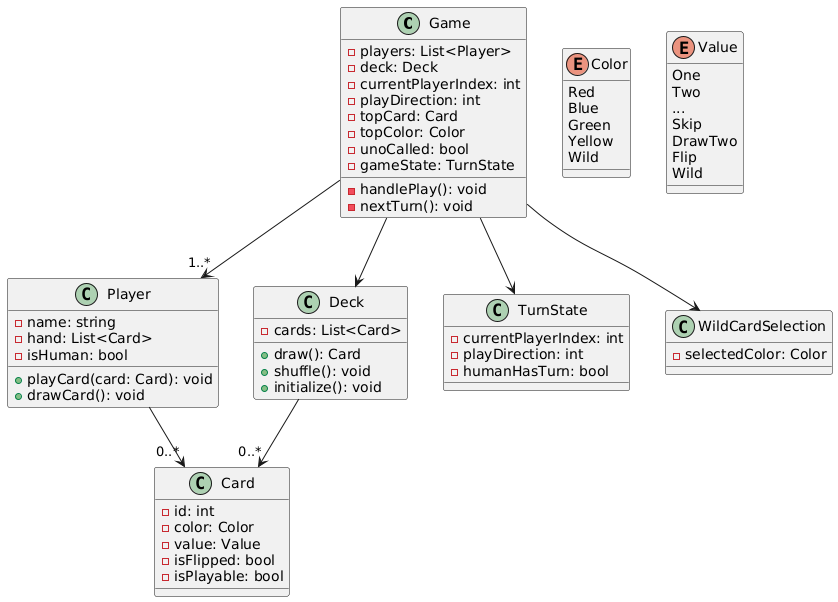
\includegraphics[width=0.9\textwidth]{business_model.png}
    \caption{Business Data Model Class Diagram}
    \label{fig:business-data-model}
\end{figure}

\subsection{Data Dictionary}
\input{data_dictionary_table.tex}

\section{The Scope of the Product}

\subsection{Product Boundary}
The UNO Flip project will deliver a multiplayer card game focused on strategic depth and AI-driven gameplay. The primary environment is a web-based platform with potential future expansion to mobile. Real-time multiplayer synchronization and dynamic card interactions are central to the experience, as well as AI opponents that can adapt and learn from gameplay. The project will not initially support offline play or mobile platforms.

\begin{figure}[H]
\centering
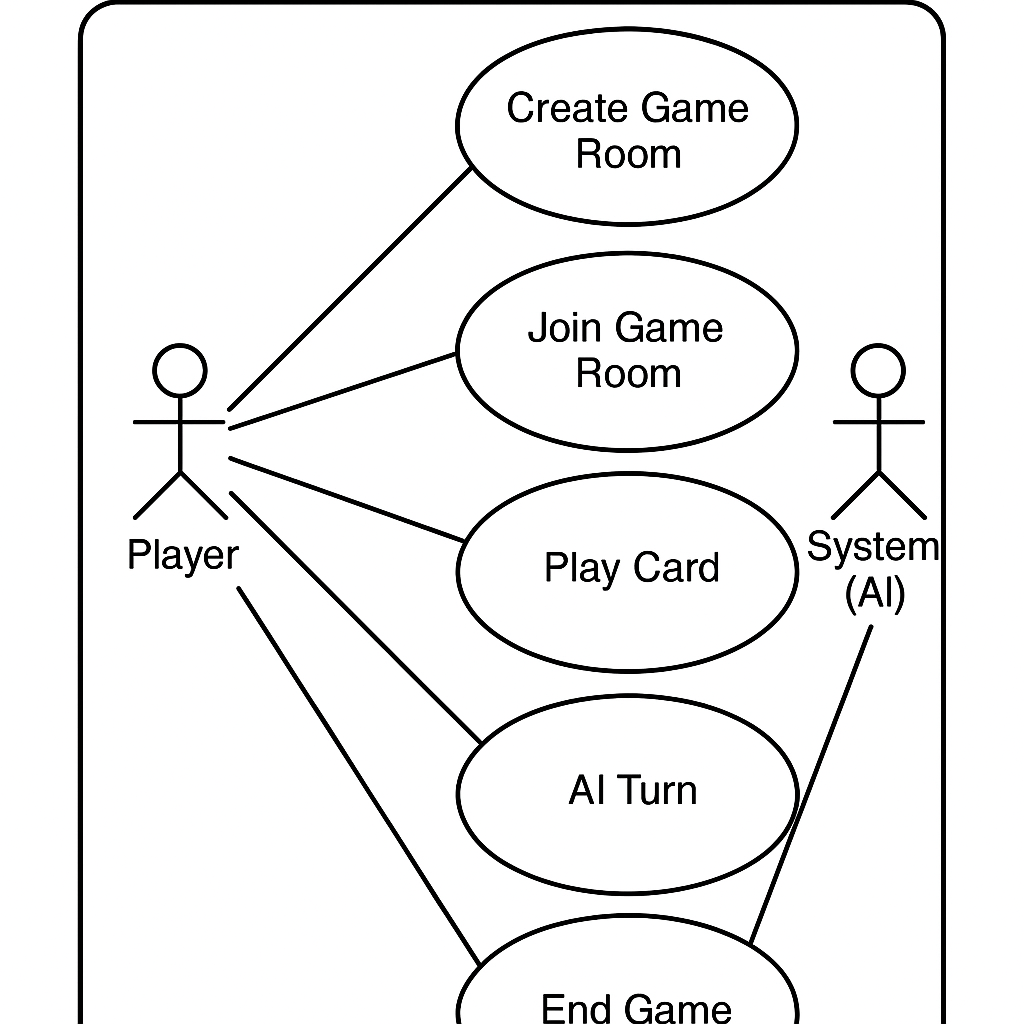
\includegraphics[width=0.7\textwidth]{PUC_diagram.png}
\caption{Use Case Diagram for UNO Flip Game}
\label{fig:usecase-diagram}
\end{figure}

\subsection{Product Use Case Table}

\begin{table}[H]
\centering
\label{tab:puc-table}
\begin{tabular}{|c|c|c|}
\hline
\textbf{ID} & \textbf{Use Case Name} & \textbf{Primary Actor} \\
\hline
UC-01 & Create Game Room & Player \\
UC-02 & Play Card & Player \\
UC-03 & AI Turn & AI Player \\
UC-04 & Call UNO & Player \\
UC-05 & End Game & System \\
\hline
\end{tabular}
\caption{Product Use Case Table}
\end{table}

\subsection{Individual Product Use Cases (PUCs)}

\textbf{UC-01: Create Game Room}

\textbf{Primary Actor:} Player

\textbf{Preconditions:}
\begin{itemize}
    \item The player has launched the game from a supported browser or system.
\end{itemize}

\textbf{Main Flow:}
\begin{enumerate}
    \item The player clicks the “Start” button from the main menu.
    \item The system prompts the player to enter a display name.
    \item The player submits a name (validated as non-empty).
    \item The system creates a new session with default game settings.
    \item The deck is shuffled, the player’s hand is dealt, and AI opponents are generated.
    \item The game begins immediately with the first turn assigned.
\end{enumerate}

\textbf{Postconditions:}
\begin{itemize}
    \item A single-player session is created, and gameplay begins with cards distributed to all players.
\end{itemize}

\textbf{Linked Requirements:} 
\begin{itemize}
    \item GSR1 — Players can create game rooms (implicitly fulfilled through the session start).
    \item TMR1 — The system initiates turn-based gameplay after setup.
    \item MSR1 — Synchronization applies locally to all in-game elements (AI/human).
\end{itemize}


\vspace{0.5cm}
\textbf{UC-02: Play Card}

\textbf{Primary Actor:} Player

\textbf{Preconditions:}
\begin{itemize}
    \item It is the player’s turn.
    \item The player has valid playable cards in their hand.
\end{itemize}

\textbf{Main Flow:}
\begin{enumerate}
    \item The player selects a card from their hand.
    \item The system checks if the card is playable.
    \item If valid, the card is played onto the discard pile.
    \item The game state updates to reflect the played card.
    \item The turn passes to the next player.
\end{enumerate}

\textbf{Postconditions:}
\begin{itemize}
    \item The game progresses to the next player.
\end{itemize}

\textbf{Linked Requirements:}
\begin{itemize}
    \item TMR1 — Turn management with state updates.
    \item MSR1 — Game state synchronized across clients.
\end{itemize}

\vspace{0.5cm}

\textbf{UC-03: AI Turn}

\textbf{Primary Actor:} System (AI)

\textbf{Preconditions:}
\begin{itemize}
    \item It is the AI’s turn.
\end{itemize}

\textbf{Main Flow:}
\begin{enumerate}
    \item The AI analyzes its hand and game state.
    \item The AI chooses a valid card to play.
    \item The system plays the card.
    \item The game state updates and continues to the next player.
\end{enumerate}

\textbf{Postconditions:}
\begin{itemize}
    \item The AI’s move is completed, and gameplay continues.
\end{itemize}

\textbf{Linked Requirements:}
\begin{itemize}
    \item TMR1 — Turn management system.
    \item MSR1 — Game synchronization for AI moves.
\end{itemize}

\vspace{0.5cm}

\textbf{UC-04: Call UNO}

\textbf{Primary Actor:} Player

\textbf{Preconditions:}
\begin{itemize}
    \item The player has exactly one card left.
    \item It is the player’s turn.
\end{itemize}

\textbf{Main Flow:}
\begin{enumerate}
    \item The player plays their second-last card.
    \item The system detects one card left in hand.
    \item The “Call UNO” button is shown.
    \item The player presses the button.
    \item The system sets \texttt{unoCalled = true}.
\end{enumerate}

\textbf{Postconditions:}
\begin{itemize}
    \item The player's UNO status is recorded for rule enforcement.
\end{itemize}

\textbf{Linked Requirements:}
\begin{itemize}
    \item TMR1 — Turn management.
    \item EGHR1 — End-game handling and win condition recognition.
\end{itemize}

\vspace{0.5cm}

\textbf{UC-05: End Game}

\textbf{Primary Actor:} System

\textbf{Preconditions:}
\begin{itemize}
    \item A player has emptied their hand of cards.
\end{itemize}

\textbf{Main Flow:}
\begin{enumerate}
    \item The system detects win condition.
    \item The system shows the end game panel.
    \item The winning player is displayed.
    \item Players may exit or replay.
\end{enumerate}

\textbf{Postconditions:}
\begin{itemize}
    \item The match ends and the results are shown.
\end{itemize}

\textbf{Linked Requirements:}
\begin{itemize}
    \item EGHR1 — Declare winner.
    \item EGHR2 — Replay or exit option.
\end{itemize}

\section{Functional Requirements}

\subsection{Functional Requirements}

\textbf{Game Initialization (GI):}
\begin{itemize}
    \item \added{GI1 - When the player clicks “Start” from the main menu, the system prompts them to enter a display name.}
    \item \added{GI2 - Upon name entry, the client connects to the TCP server and joins a multiplayer session.}
    \item \added{GI3 - When the required number of players have joined, the server deals 7 cards to each player and begins the match.}
    \item \removed{AR1 - Players must log in or create an account to access multiplayer modes.}
    \item \removed{AR2 - User profiles will store game statistics and preferences.}
\end{itemize}

\textbf{Multiplayer Turn Management (MTM):}
\begin{itemize}
    \item \added{MTM1 - The server maintains turn order using a synchronized index and direction, and broadcasts it to all clients.}
    \item \added{MTM2 - The active player receives a notification when it is their turn.}
    \item \added{MTM3 - The server enforces turn order, rejecting out-of-turn moves.}
    \item \removed{TMR1 - The system will manage player turns, ensuring synchronization across devices.}
    \item \removed{TMR2 - Notifications will alert players when it is their turn.}
\end{itemize}

\textbf{Card Play (CP):}
\begin{itemize}
    \item \added{CP1 - When a player attempts to play a card, the client sends a play request to the server.}
    \item \added{CP2 - The server checks if the card is playable according to Uno Flip rules.}
    \item \added{CP3 - If the card is valid, the server updates the game state and informs all players.}
    \item \added{CP4 - Special cards (Skip, Reverse, Draw cards, Flip) trigger their respective effects.}
    \item \added{CP5 - When a Flip card is played, the deck and all player hands switch between light and dark sides.}
\end{itemize}

\textbf{UNO Declaration (UD):}
\begin{itemize}
    \item \added{UD1 - When a player has one card left, they must press the “UNO” button.}
    \item \added{UD2 - If the player fails to declare UNO and another player catches it, the system penalizes them with 2 cards.}
\end{itemize}

\textbf{AI Behavior (AIB):}
\begin{itemize}
    \item \added{AIB1 - AI players are added at game creation if selected.}
    \item \added{AIB2 - AI logic selects a valid card based on rule-based logic and submits it to the server.}
    \item \added{AIB3 - The AI can declare UNO and react to wild and special cards correctly.}
    \item \removed{GSR2 - Options for choosing game rules and difficulty settings.}
\end{itemize}

\textbf{End Game Handling (EGH):}
\begin{itemize}
    \item \added{EGH1 - The server checks after each turn whether a player has emptied their hand.}
    \item \added{EGH2 - When a win condition is detected, the server announces the winner and ends the session.}
    \item \removed{EGHR1 - The game will automatically declare a winner based on the rules and display a summary of the results.}
    \item \removed{EGHR2 - Players can choose to play another round or exit the game.}
\end{itemize}

\textbf{Multiplayer Synchronization (MS):}
\begin{itemize}
    \item \added{MS1 - After each action (e.g., card played, card drawn, turn ended), the server sends the updated game state to all clients.}
    \item \added{MS2 - The client UI updates automatically upon receiving new game state data.}
    \item \added{MS3 - If a player disconnects, the server handles the event gracefully and continues the match.}
    \item \removed{MSR1 - A state synchronization mechanism will ensure that all players see the same game state at all times, regardless of network conditions.}
    \item \removed{MSR2 - The system will manage latency and update the game state in real time.}
\end{itemize}

\added{\textbf{Game Rule Enforcement}
\begin{itemize}
    \item GRE1 - The system shall enforce all UNO Flip rules, including the behavior of flip, skip, reverse, wild draw, and color switch cards.
    \item GRE2 - The current game state (front or back) must change only on a Flip card and be visible to all players.
    \item GRE3 - The system must prevent illegal card plays based on current color, number, or game side.
\end{itemize}}

\textbf{Removed Features (Not Implemented):}
\begin{itemize}
    \item \removed{CFR1 - Real-time chat within the game room for players to communicate.}
    \item \removed{CFR2 - Chat can be enabled or disabled based on player preferences.}
    \item \removed{SSR1 - A detailed scoring mechanism to track and display player scores at the end of each game.}
    \item \removed{SSR2 - The system will keep a record of player stats, including wins, losses, and average score.}
\end{itemize}

\section{Look and Feel Requirements}

\subsection{Appearance Requirements}
\begin{itemize}
    \item \removed{AR1 - The game interface should have a modern design that is visually appealing.}
    \item \added{AR1 - The game interface must follow a modern, minimalistic design using clean fonts, bold colors, and flat UI components.}
    \item AR2 - Consistency in color schemes, fonts, buttons, and animation effects should be maintained throughout the game.
    \item \removed{AR3 - Card designs should be easily recognizable, with clarity maintained during 3D rendering.}
    \item \added{AR3 - Card designs must be large, legible, and aligned with the official UNO Flip theme (dual-sided cards with unique colors and symbols).}
    \item \added{AR4 - Turn direction and current player status should be clearly visualized through directional arrows and on-screen messages.}
\end{itemize}


\subsection{Style Requirements}
\begin{itemize}
    \item \removed{SR1 - The interface should be adaptive, ensuring proper display on different screen resolutions for mobile, tablet, and desktop devices.}
    \item \added{SR1 - The interface is optimized for PC screens only. Support for mobile and tablet devices is not available in the current version.}
    \item SR2 - Actions in the game (e.g., flipping a card, playing a card) should feature smooth and responsive animations.
    \item \added{SR3 - Game elements (cards, buttons, player indicators) must respond to user input with minimal latency.}
\end{itemize}

\section{Usability and Humanity Requirements}

\subsection{Ease of Use Requirements}
\begin{itemize}
    \item \removed{EOUR1 - New players should be able to quickly grasp the gameplay, with the system providing simple and clear tutorials.}
    \item \added{EOUR1 - New players should understand core gameplay within 1–2 turns, supported by an optional on-screen rule summary.}
    \item \removed{EOUR2 - The game menu and control buttons should be easy to navigate, allowing players to easily create or join rooms.}
    \item \added{EOUR2 - The game menu and control buttons must support mouse input, large buttons, and minimal nested navigation.}
    \item \removed{EOUR3 - Drag-and-drop actions for playing cards should be intuitive and highly responsive.}
    \item \added{EOUR3 - Playing cards must require a simple click action. Drag-and-drop is not implemented.}
\end{itemize}

\subsection{Personalization and Internationalization Requirements}
\begin{itemize}
    \item \removed{PALR1 - The game should support language localization, offering options for multiple languages (e.g., English, French, Spanish).}
    \item \added{PALR1 - The game is currently available in English only. Multilingual support is a potential future enhancement.}
    \item \removed{PALR2 - Players can customize personal settings, such as sound effects, background music, and interface themes, for a personalized experience.}
    \item \added{PALR2 - Players can adjust basic game visuals such as resolution and full-screen mode.}
\end{itemize}

\subsection{Learning Requirements}
\begin{itemize}
    \item \removed{LR1 - The system will offer interactive tutorials for new players to understand the rules of UNO Flip and the effects of special cards.}
    \item \added{LR1 - The game includes brief, non-interactive rule reminders for special cards at the start of the game.}
    \item \removed{LR2 - AI will guide players to familiarize themselves with advanced strategies and dynamically adjust difficulty based on player performance.}
    \item \added{LR2 - AI behavior is rule-based and does not change in response to player actions.}
\end{itemize}

\subsection{Understandability and Politeness Requirements}
\begin{itemize}
    \item \added{UAFR1 - All system messages use short, friendly phrases like “Your Turn” or “UNO!” to maintain accessibility.}
    \item \added{UAFR2 - A rules panel or help menu is available to review gameplay expectations during play.}
    \item \added{UAFR3 - The system must support both casual play (quick matches with AI) and competitive sessions with stat tracking, to appeal to different player types.}

\end{itemize}

\subsection{Accessibility Requirements}
\begin{itemize}
    \item \removed{AR1 - The game should support accessibility features such as colorblind modes, text enlargement options, and a soundless mode for hearing-impaired users.}
    \item \added{AR1 - Accessibility support such as colorblind mode or text resizing is not implemented in the current version.}
    \item \removed{AR2 - For mobile devices, the game should support multi-touch controls and be compatible with accessibility devices.}
    \item \added{AR2 - The interface is optimized for keyboard and mouse use on desktop environments.}
\end{itemize}

\section{Performance Requirements}

\subsection{Speed and Latency Requirements}
\begin{itemize}
    \item SALR1 - The average response time for the game should be within 50 milliseconds to ensure smooth interaction.
    \item SALR2 - Network latency in multiplayer mode should be kept under 200 milliseconds to avoid inconsistencies in the game state.
\end{itemize}

\subsection{Safety-Critical Requirements}
\begin{itemize}
    \item SCR1 - Changes in the card and game state must be synchronized in real-time to ensure all players see the same status.
    \item SCR2 - Disaster recovery mechanisms should be in place to save game progress and resume play in case of server failure.
\end{itemize}

\subsection{Precision or Accuracy Requirements}
\begin{itemize}
    \item POAR1 - When calculating scores and game state, the system should ensure high precision to avoid incorrect scorekeeping or errors in the game logic.
\end{itemize}

\subsection{Robustness or Fault-Tolerance Requirements}
\begin{itemize}
    \item ROFR1 - The system should be fault-tolerant, allowing players to reconnect quickly after a network interruption without losing game progress.
    \item ROFR2 - The server should handle a surge in user logins without crashing.
\end{itemize}

\subsection{Capacity Requirements}
\begin{itemize}
    \item CP1 - The system should support at least 1,000 concurrent users, with each game room running independently.
    \item CP2 - Each game room should support up to 4 to 8 players.
\end{itemize}

\subsection{Scalability or Extensibility Requirements}
\begin{itemize}
    \item SOER1 - The system should be scalable, allowing for future additions of new game modes, features, or AI difficulty levels.
    \item SOER2 - As the player base grows, the server should be able to scale dynamically to handle more concurrent users.
\end{itemize}

\subsection{Longevity Requirements}
\begin{itemize}
    \item LR1 - The game’s code should be maintainable for long-term use, supporting future updates, performance optimizations, and feature expansions.
\end{itemize}

\section{Operational and Environmental Requirements}

\subsection{Expected Physical Environment}
\begin{itemize}
    \item EPER1 - The system will primarily run on desktop and laptop platforms (Windows, macOS) using modern web browsers.
\end{itemize}

\subsection{Wider Environment Requirements}
\begin{itemize}
    \item WER1 - The game must perform under varying network speeds, implementing latency mitigation techniques such as rollback networking to ensure smooth gameplay even in slower or unstable connections.
    \item WER2 - The game must detect internet interruptions and allow players to reconnect without losing game progress.
    \item WER3 - The game must be compatible with all major web browsers (Chrome, Firefox, Safari, and Edge).
\end{itemize}

\subsection{Requirements for Interfacing with Adjacent Systems}
\begin{itemize}
    \item RFIWASR1 - The game must integrate with third-party authentication providers (e.g., Google, Facebook) to allow users to log in using existing accounts.
    \item RFIWASR2 - The game should integrate with social media platforms for sharing gameplay results or achievements.
\end{itemize}

\subsection{Productization Requirements}
\begin{itemize}
    \item PR1 - The game must undergo thorough testing across multiple devices, browsers, and network conditions to ensure consistent performance and identify any compatibility issues.
    \item PR2 - The system must undergo performance optimization to handle at least 1,000 concurrent users across different multiplayer rooms.
\end{itemize}

\subsection{Release Requirements}
\begin{itemize}
    \item RR1 - The initial release must include a robust help system, including in-game tutorials and access to FAQs or troubleshooting guides.
    \item RR2 - The system must support post-launch patches and updates without requiring users to reinstall or experience significant downtime.
    \item RR3 - The release version must undergo comprehensive regression testing to ensure that all core functionalities work as expected across devices and browsers.
\end{itemize}

\section{Maintainability and Support Requirements}

\subsection{Maintenance Requirements}
\begin{itemize}
    \item MR1 - The game must maintain a frame rate of at least 30 FPS across all supported platforms, ensuring smooth animations and interactions.
    \item MR2 - The system must support up to 1,000 concurrent users in multiplayer mode without significant degradation in performance or user experience.
    \item MR3 - Actions taken by players, such as playing or drawing a card, must occur in under 500 milliseconds to avoid noticeable delays in gameplay.
\end{itemize}

\subsection{Supportability Requirements}
\begin{itemize}
    \item SR1 - The system should offer online technical support, and players should be able to report issues in-game or via the website.
    \item SR2 - The system must detect and recover from unexpected disconnections, allowing players to resume gameplay within 10 seconds of a reconnection.
\end{itemize}

\subsection{Adaptability Requirements}
\begin{itemize}
    \item AR1 - The system must ensure 24/7 availability for users worldwide, with planned downtime limited to maintenance windows of no more than 2 hours per month.
    \item AR2 - Maintenance and updates must be rolled out during off-peak hours to minimize disruption to users.
    \item AR3 - The game must include an offline maintenance mode where players can still practice against AI when the server is unavailable.
\end{itemize}

\section{Security Requirements}

\subsection{Access Requirements}
\begin{itemize}
    \item AR1 - Players must securely log in to the game, with support for two-factor authentication (2FA) for added security.
    \item AR2 - The game should have a password recovery mechanism to allow users to recover their passwords in case they forget them.
\end{itemize}

\subsection{Integrity Requirements}
\begin{itemize}
    \item IR1 - All player data (such as game progress and personal stats) should be encrypted to prevent unauthorized modification.
    \item IR2 - The game should not allow weak passwords (e.g., passwords composed only of numbers or letters) for login credentials.
\end{itemize}

\subsection{Privacy Requirements}
\begin{itemize}
    \item PR1 - Player data (such as personal information and game records) should comply with privacy policies to prevent data breaches.
    \item PR2 - The game should notify users that they should not share their personal information with others in the game room.
    \item PR3 - The game should automatically log users out after a certain period of inactivity to prevent unauthorized access.
\end{itemize}

\subsection{Audit Requirements}
\begin{itemize}
    \item AR1 - The system should log all critical operations in the backend to allow for auditing and troubleshooting.
    \item AR2 - In case of frontend crashes, the game should provide crash information to the backend for future improvements (with user consent).
\end{itemize}

\subsection{Immunity Requirements}
\begin{itemize}
    \item IR1 - The system should be immune to common network attacks (e.g., DDoS, SQL injection) to ensure the safety of player data and gameplay.
    \item IR2 - The system should be resilient to network issues, such as fluctuations in connection speed.
\end{itemize}

\section{Cultural Requirements}

\subsection{Cultural Requirements}
\begin{itemize}
    \item CR1 - The game should be adapted to global markets, avoiding cultural sensitivities and contentious topics.
    \item CR2 - The content and language shown in the game should not be offensive to any particular culture.
    \item CR3 - The game should respect the cultural customs and religious doctrines of the countries where it is released.
\end{itemize}

\section{Compliance Requirements}

\subsection{Legal Requirements}
The UNO Flip Remix project must comply with data protection regulations such as the \href{https://gdpr.eu/}{General Data Protection Regulation (GDPR)} for European users and the \href{https://oag.ca.gov/privacy/ccpa}{California Consumer Privacy Act (CCPA)} for users in California. In addition, the project should align with the content guidelines established by the \href{https://www.esrb.org/ratings-guide/}{Entertainment Software Rating Board (ESRB)} to ensure age-appropriate content for general audiences.

This requires the game to implement robust data protection measures, including encryption for personal data, secure storage practices, and mechanisms to obtain explicit user consent for data collection and processing. User rights, such as the ability to access, rectify, or delete their personal information, must be respected, with clear procedures for users to exercise these rights. Privacy policies must be transparent, detailing the types of data collected, purposes for data processing, and third-party data sharing practices.



\subsection{Standards Compliance Requirements}
\begin{itemize}
    \item SCR1 - The game must comply with international standards and local laws, especially regarding data protection regulations such as \href{https://gdpr.eu/}{GDPR}, \href{https://oag.ca.gov/privacy/ccpa}{CCPA}, and content rating guidelines outlined by the \href{https://www.esrb.org/}{Entertainment Software Rating Board (ESRB)}.

    \item SCR2 - The system’s development should adhere to industry best practices for code quality and testing.
\end{itemize}

\section{Open Issues}
Several open issues need to be resolved as the project progresses:
\begin{itemize}
    \item The decision between a rule-based AI and reinforcement learning remains unresolved and will directly impact both the performance and development timeline. 
    \added{Related to requirements: LR2, PR1, SOER1}

    \item Ensuring smooth real-time synchronization in multiplayer mode as the number of concurrent players increases will require further testing, particularly with network latency. 
    \added{Related to requirements: SALR2, ROFR1, WER1}

    \item Cross-platform support for mobile devices presents challenges, particularly in optimizing the user interface and game performance for mobile networks. 
    \added{Related to requirements: SR1, WER2, AR1, AR2}
\end{itemize}

\section{Off-the-Shelf Solutions}

\subsection{Ready-Made Products}
The UNO Flip Remix project will utilize several existing software solutions to expedite the development process and ensure a high-quality gaming experience:
\begin{itemize}
    \item \removed{\textbf{TensorFlow:} Employed for integrating AI functionalities, TensorFlow will power the decision-making process for AI opponents, providing a more challenging and dynamic gameplay experience.}
    \item \removed{\textbf{Socket.IO:} Used for real-time communication, this framework ensures smooth synchronization across players during multiplayer sessions, minimizing latency.}
    \item \added{\textbf{Custom TCP Server (C\#):} A Unity-compatible C\# server is used for managing real-time multiplayer communication, ensuring synchronization across players and handling connection logic.}
    \item \textbf{Firebase:} This cloud-based solution will be leveraged for data storage and user management, including game data, player profiles, and session management.
    \item \removed{\textbf{3D Graphics Libraries (e.g., Three.js):} Libraries like Three.js will facilitate the rendering of 3D elements, animations, and lighting effects, enhancing the visual experience of the game.}
    \item \added{\textbf{Unity Game Engine:} The game is built using Unity’s 2D capabilities, handling rendering, input, physics, and scene management.}
\end{itemize}

\subsection{Reusable Components}
To improve efficiency and ensure high-quality outcomes, the following reusable components will be incorporated:
\begin{itemize}
    \item \removed{ 3D Game Frameworks such as Three.js for creating 3D objects, animations, and scene management.}
    \item \textbf{Authentication Libraries (e.g., Firebase Auth):} Used for implementing user login, session tracking, and account management.
    \added{\item \textbf{Rule-Based AI Templates:} Predefined logic for AI card selection and game behavior, used in lieu of machine learning approaches.}
    \item \textbf{UI/UX Frameworks (Unity UI):} Unity’s UI toolkit is used for menus, buttons, animations, and transitions.
\end{itemize}
\subsection{Products That Can Be Copied}
The existing version of the UNO Flip game available at \url{https://unoonlinegame.io/uno-flip-online} serves as a reference for this project. While it provides a functional basis, the UNO Flip Remix project aims to improve its visuals, gameplay flow, and features.
\begin{itemize}
    \item \removed{\textbf{Visual Overhaul:} The current game's simplistic graphics will be replaced with a more dynamic 3D presentation, including card animations and interactive game boards.}
    \item \added{\textbf{Visual Enhancements:} The current game's 2D visuals will be enhanced with improved sprite design, transitions, and polished animations.}
    \item \textbf{Enhanced Gameplay Flow:} The game will be improved with smoother transitions, refined animations, and interactive elements for a more responsive and exciting gameplay experience.
    \item \removed{\textbf{Additional Features:} Modern features like real-time lighting effects, dynamic sound design, and fluid animations will enhance the overall user experience.}
    \item \added{\textbf{Additional Features:} Features such as rule-based AI, real-time multiplayer, and UNO Flip-specific mechanics will enrich the gameplay.}
\end{itemize}

\section{New Problems}

\subsection{Effects on the Current Environment}
The transition from a physical card game to a digital interface introduces several challenges:
\begin{itemize}
    \item Players who are accustomed to the physical version may face a learning curve with the digital interface. \added{This is mitigated by EOUR1 and LR1 which aim to reduce the barrier to entry.}
    \item The game’s dependency on stable internet connections means that network interruptions can disrupt gameplay, unlike the offline nature of physical card games. \added{Covered by ROFR1 and SR2.}
\end{itemize}

\subsection{Effects on Installed Systems}
\begin{itemize}
    \item \removed{Ensuring cross-platform compatibility across devices such as desktops, laptops, and mobile devices will require system optimizations and updates.}
    \item \added{Ensuring compatibility with different desktop environments (Windows/macOS) may require additional UI scaling and resolution testing.}
    \item Security measures like anti-cheating systems may require updates to prevent manipulation of online scores or game states. \added{This relates to IR1 and IR2.}
\end{itemize}

\subsection{Potential User Problems}
\begin{itemize}
    \item Users unfamiliar with the digital interface might struggle with game controls, such as flipping cards. \added{This is addressed by EOUR3 and LR1.}
    \item In-game cheating could become a problem, requiring robust security measures to ensure fair play. \added{This ties into IR1 and AR1.}
    \item Disconnected sessions due to network issues might cause frustration, especially in competitive gameplay. \added{Covered by ROFR1, SR2.}
\end{itemize}

\subsection{Limitations in the Anticipated Implementation Environment That May Inhibit the New Product}
\begin{itemize}
    \item Players with slow or unstable internet connections may experience lag or interruptions in gameplay. \added{(SALR2, ROFR2)}
    \item \removed{Low-end devices may struggle with handling the game’s 3D graphics and real-time multiplayer synchronization.}
    \item \added{Low-end devices may struggle with Unity-based rendering or network message processing during peak load.}
    \item Synchronization across devices with varying performance capabilities may lead to discrepancies in game experience. \added{This is handled through MSR1 and SALR1.}
\end{itemize}

\subsection{Follow-Up Problems}
\begin{itemize}
    \item Regular updates and patches may be required to address bugs, introduce new features, or balance the game mechanics, without breaking the existing functionality. \added{(LR1, PR2)}
    \item Long-term player retention may depend on the addition of new content and features to keep the game engaging and competitive. \added{(SOER1, CR3)}
\end{itemize}

\section{Tasks}

\subsection{Project Planning}
Our team will hold weekly meetings to track progress and align on project tasks. Each team member is expected to attend these meetings. Additionally, we will organize informal work sessions throughout the week to collaborate on specific tasks and document our progress. \\

\textbf{Weekly Scrum meetings:}
\begin{itemize}
    \item Weekly Scrum meetings will be conducted with all team members attending.
    \item Each meeting will last between 15 and 30 minutes and will occur on Microsoft Teams.
    \item Members will discuss progress and any blockers encountered. 
    \item \added{The Scrum Master will update the backlog and burn-down chart to track task progress.}
    \item \added{Retrospective meetings will occur every two weeks to reflect on progress and adjust team workflows.}
\end{itemize}

\textbf{Additional work sessions:}
\begin{itemize}
    \item At least one additional work session per week will be held where coding and design tasks will be conducted collaboratively.
\end{itemize}

Primary communication will occur on Microsoft Teams, supplemented by cell phone coordination when necessary. The team will also utilize GitHub for version control and code reviews.

\subsection{Planning of the Development Phases}
The project will follow a Git-flow branching model to streamline development and ensure effective collaboration among team members. In this model, each new feature or bug fix will be developed in its own dedicated branch. This approach allows for focused work on individual components without disrupting the main codebase.

Once a feature is completed, team members will submit a pull request to merge their changes into the master branch. Each pull request will undergo a review process where other team members can provide feedback, suggest improvements, and identify potential issues before integration. This collaborative review process enhances code quality and promotes knowledge sharing within the team.

\added{To phase in development based on priority:}
\begin{itemize}
    \item \added{Phase 1 will implement core game mechanics and multiplayer (FR1–FR5, MTM1–MTM3).}
    \item \added{Phase 2 will focus on UI/UX design and accessibility (UIR1–UIR3, ACR1–ACR2).}
    \item \added{Phase 3 will address scoring, end game logic, and player statistics (SC1–SC3, EGH1–EGH2).}
    \item \added{Phase 4 will refine AI behavior and game balance (AI1–AI3).}
    \item \added{Phase 5 will add extra features such as colorblind mode, input tuning, and performance optimization (A11Y1, SALR1, ROFR1).}
\end{itemize}

\added{Each module will include automated unit tests to verify behavior, ensuring traceability to its associated functional or non-functional requirements (see Section 22).} Unit testing will validate the reliability and functionality of our code. These tests will be written alongside the code and run regularly to catch regressions early in the development process. \added{The team will also document requirement-to-test mappings in the Traceability Matrix.}

\section{Migration to the New Product}

\subsection{Requirements for Migration to the New Product}
\begin{itemize}
    \item \textbf{Data Integration:} Existing player data, including usernames, scores, and progress from any prototype or beta versions, must be seamlessly integrated into the new system. \added{This links to requirement SC3.}
    
    \item \textbf{System Compatibility:} \removed{The new digital platform should be compatible with various devices (desktop, mobile, and tablet)} \added{The new digital platform should support major desktop and laptop browsers (Windows/macOS) only} to ensure a consistent user experience across all platforms. \added{Linked to ENVR1 and ENVR3.}
    
    \item \textbf{User Authentication and Data Security:} Secure authentication mechanisms must be in place to protect user accounts and personal information. Existing authentication data may need to be encrypted or reformatted to meet new security standards. \added{(Linked to SEC1 and SEC3).}
    
    \item \removed{\textbf{AI Implementation Adaptation:} The AI behavior from the initial rule-based prototype needs to be adapted and optimized for the TensorFlow-based reinforcement learning model planned for the new system.} \added{\textbf{AI Implementation Migration:} The initial rule-based AI logic will be retained and refactored for use in the production multiplayer setting. This supports AI1–AI3.}
    
    \item \textbf{Rollback Networking Technique:} The implementation of rollback networking techniques must be tested and adjusted to maintain real-time synchronization in multiplayer sessions, ensuring that latency issues are minimized during gameplay. \added{(Linked to MTM3 and MTM4).}
    
    \item \textbf{Training and Support:} Detailed documentation and tutorials should be provided to users to guide them through the features of the new digital version, emphasizing the differences between the physical and digital gameplay experiences. \added{(Supports UX3 and LR1).}
\end{itemize}

\subsection{Data That Has to be Modified or Translated for the New System}
\begin{itemize}
    \item \textbf{Data Format Transformation:} Data from the original or prototype version of the UNO Flip game, including card decks, player profiles, and game history, may need to be reformatted to match the new system's data schema. \added{(Linked to SC1 and GI2).}
    
    \item \textbf{User Profile Data:} Existing user data, such as login credentials, player stats, and in-game achievements, must be translated into a format compatible with the new authentication and storage standards used by the digital platform. \added{(Linked to SEC2 and SC2).}
    
    \item \removed{\textbf{AI Training Data:} Historical gameplay data should be converted into training datasets for the TensorFlow-based AI. This data must be processed to suit the specific input format required for reinforcement learning algorithms.}
    
    \item \textbf{Card Interaction Logic:} The logic governing card interactions and game rules from the traditional version should be modified to fit the digital framework, ensuring that the new system accurately replicates the physical gameplay mechanics. \added{This directly supports GI1–GI3 and ENDR1.}
    
    \item \textbf{Multiplayer Session Data:} Information related to multiplayer sessions, such as game states and player interactions, must be adapted \removed{to function within the Socket.IO framework} \added{to function within the custom TCP server framework} to enable real-time communication and synchronization. \added{(Supports MTM2–MTM4).}
\end{itemize}

\section{Costs}

\begin{table}[H]
\centering
\begin{tabular}{|p{3.5cm}|p{8.5cm}|p{2cm}|}
\hline
\textbf{Item} & \textbf{Details} & \textbf{Cost} \\
\hline
Cloud Hosting (Server) & Hosting multiplayer TCP game sessions and backend services. \added{This supports requirements MTM1–MTM4 and SEC1.} & \$100 \\
\hline
Data Storage & \removed{Firebase for data storage and user management.} \added{Cloud-based database (e.g., Supabase or custom TCP logs) for storing user profiles and match data. Supports SC1–SC3.} & \$50 \\
\hline
\removed{Graphics Support (API)} & \removed{Possible need for graphic APIs (e.g., OpenGL) for 3D effects.} & \removed{\$20–\$70} \\
\hline
Unity Assets & \added{Free or low-cost Unity assets (e.g., card images, UI packs) to speed up 2D development.} & \$0–\$30 \\
\hline
\end{tabular}
\caption{Estimated Project Costs}
\end{table}

\section{User Documentation and Training}

\subsection{User Documentation Requirements}
\begin{itemize}
    \item UDR1 - A visual guide to the game’s user interface, covering controls for card selection, flipping between sides, and accessing in-game settings.
    \item \removed{UDR2 - A section addressing common issues, such as resolving connection problems, understanding game mechanics, and how scoring works.}
    \item \added{UDR2 - A guide to connection troubleshooting, scoring logic, and digital-specific interactions in UNO Flip (e.g., flip mechanic, wild draw color behavior).}
    \item UDR3 - \removed{Basic troubleshooting steps for resolving common issues, such as server disconnects or game freezes.} \added{Common troubleshooting tips for network disconnects and turn desync in multiplayer.}
\end{itemize}

\subsection{Training Requirements}
\begin{itemize}
    \item TR1 - New players will be guided through a hands-on, in-game tutorial that explains game rules, mechanics, and card effects in real-time. \added{This will ensure clarity between traditional UNO and UNO Flip mechanics.}
    \item TR2 - A help section within the game, accessible at any time, will provide reminders of the rules and descriptions of card functions.
    \item TR3 - Players can practice in solo mode against AI opponents before entering multiplayer matches to get familiar with the interface and rules. \added{This supports onboarding for both casual and enthusiast players.}
\end{itemize}

\section{Waiting Room}
The following features and functionalities may be considered as future stretch goals as outlined in the development plan:

\begin{itemize}
    \item \removed{Advanced AI using reinforcement learning for more sophisticated gameplay.}
    \item \added{More complex AI logic to simulate adaptive strategies and player behavior may be added in future versions.}
    
    \item Mobile App Version: Focus on a web-based platform in the current phase, with mobile app development to be explored later. \added{This will require interface scaling and compatibility testing.}
    
    \item Cross-Platform Play: Potential future support for players on different devices to play together. \added{Would require input normalization and multiplayer synchronization adjustments.}
    
    \item In-Game Purchases: Monetization through in-game purchases or microtransactions is not planned for this phase. \added{This will need to comply with monetization guidelines and possibly ESRB age-rating standards.}
    
    \item Offline Play: The game will require a continuous internet connection; offline play will be considered in later versions. \added{A local AI-only game loop would need to be supported.}
    
    \item Custom Game Modes: Future iterations may introduce customizable or additional game modes. \added{Rule configuration UI and alternate game logic pipelines would be required.}
    
    \item Voice Chat Integration: Text-based chat functionality will be implemented, with voice chat considered for future releases. \added{May require integration with third-party VoIP APIs and moderation tooling.}
    
    \item Network Latency Optimization: \removed{Advanced latency management techniques (e.g., rollback networking) will be explored in future updates.}
    \item \added{Further improvements to latency handling may be explored through rollback or input prediction methods.}
    
    \item Scalability for Larger Games: The system will initially support a limited number of players, with larger capacities to be considered later. \added{May involve server-side refactoring and lobby session restructuring.}
\end{itemize}

\section{Ideas for Solution}
The UNO Flip Remix project will include the following features and functionalities:
\begin{itemize}
    \item Player Authentication: Users can create accounts, log in, and manage their profiles.
    \item Multiplayer Functionality: Players can create or join game rooms to compete in real-time against other human players.
    \item Turn Management: The game will follow the turn-based rules of UNO Flip, ensuring proper synchronization and validation of each player's moves.
    \item Basic AI Opponents: AI-controlled players will be available to fill game rooms or provide an alternative to multiplayer.
    \item Chat Functionality: Players will have access to an in-game chat system for communication during matches.
    \item Scoring System: A scoring mechanism will track player performance throughout each match.
    \item End Game Handling: The system will handle end-game scenarios, announcing winners and displaying game statistics.
    \item Multiplayer Synchronization: The game state will be synchronized across all clients in real-time, ensuring consistent gameplay for all players.
\end{itemize}

\subsection{Likely Changes}
Based on the current implementation and Section 27, the following functionalities are subject to potential change:
\begin{itemize}
    \item \textbf{Chat Functionality}: \added{This feature may be removed or limited to predefined messages if development time is constrained or moderation becomes a concern.}
    
    \item \textbf{Basic AI Opponents}: \added{While currently implemented as rule-based, their complexity and behavior may be simplified or enhanced depending on playtesting feedback and available time.}
    
    \item \textbf{Authentication Mechanism}: \added{User login may shift from full account creation to lightweight guest sessions if simplicity or accessibility becomes a higher priority.}
\end{itemize}

\subsection{Unlikely Changes}
These features are considered core to the gameplay experience and are unlikely to be changed:
\begin{itemize}
    \item \textbf{Multiplayer Functionality}: \added{As the foundation of the game experience, this is essential for enabling player interaction. (Supports MTM1–MTM4)}
    
    \item \textbf{Turn Management}: \added{The game logic requires strict turn validation to enforce UNO Flip rules. (Supports RGL1–RGL4)}
    
    \item \textbf{Scoring System}: \added{Required for determining outcomes and tracking player progress. (Supports SC1–SC2)}
    
    \item \textbf{End Game Handling}: \added{Must provide clear feedback and results at the conclusion of each match. (Supports EG1)}
    
    \item \textbf{Multiplayer Synchronization}: \added{Essential for consistency and fairness in real-time sessions. (Supports MTM3–MTM4)}
\end{itemize}

\section{Appendix — Reflection}
The information in this section will be used to evaluate the team members on the graduate attribute of Lifelong Learning. Please answer the following questions:

\subsection{Reflection Questions and Responses}

\textbf{1. What knowledge and skills will the team collectively need to acquire to successfully complete this capstone project?}

None of us had worked with Unity before starting this project, so we all had to learn the fundamentals of Unity development from scratch. As a team, we needed to acquire knowledge in the following areas:
\begin{itemize}
    \item Unity Game Engine basics — understanding the editor, working with scenes, and scripting in C#.
    \item Multiplayer game development using TCP servers — setting up client-server architecture and maintaining synchronization.
    \item Creating a responsive and intuitive user interface with animations for smooth gameplay.
    \item Following good software engineering practices like version control with Git, writing modular code, and documenting our progress clearly.
\end{itemize}

\textbf{2. For each of the knowledge areas and skills identified, what are at least two approaches to acquiring the knowledge or mastering the skill? Of the identified approaches, which will each team member pursue, and why did they make this choice?}

Since we all needed to get comfortable with Unity, we decided that each team member would take on a different focus based on their role in the project. Here's how we approached learning:

\begin{itemize}
    \item \textbf{Kevin:} I focused on gameplay programming and AI. I looked at Unity tutorials on scripting and spent time reading through open-source card games on GitHub. I chose this approach because it helped me see how actual Unity projects structure their game logic — especially for turn-based games.

    \item \textbf{Mingyang:} My main focus was backend networking. I read C# TCP server examples and studied how to connect Unity clients to external servers. I picked this approach because we’re using a custom TCP server rather than Unity's built-in networking tools, and I wanted to make sure I understood how it all worked.

    \item \textbf{Jianhao:} I worked on the UI and user experience. I followed Unity's UI Toolkit documentation and spent time prototyping layouts using Canvas and prefab buttons. Experimenting directly in Unity helped me figure out what felt intuitive from a user perspective.

    \item \textbf{Zain:} I focused on documentation and coordinating the overall system. I reviewed example SRS and VnV documents, and I regularly synced with the rest of the team to understand what was being implemented. This helped me keep the documents aligned with the actual state of the project.
\end{itemize}

As a group, we learned through a mix of tutorials, trial and error, and constant collaboration. We regularly helped each other troubleshoot and shared resources, which made the learning process smoother for everyone.

\section{Revision History}
\begin{tabularx}{\textwidth}{|c|c|X|}
\hline
\textbf{Revision Number} & \textbf{Name} & \textbf{Notes} \\
\hline
Revision 0 & Kevin Ishak and Mingyang Xu & Created first draft \\
Revision 1 & Mingyang Xu and Jianhao Wei & Added functional and non-functional requirements \\
Revision 2 & Mingyang Xu and Jianhao Wei & Added functional and non-functional requirements \\
Revision 3 & Andy Liang & Updated Terms, Acronyms and Abbreviations \\
Revision 4 & Zain-Alabedeen Garada & Updated sections 8, 13, 14 and 18. \\
\added{Revision 5} & \added{Kevin Ishak} & \added{Reviewed and addressed all TA feedback in detail. Revised every section as necessary, updated references, clarified ambiguities, added traceability, fixed formatting, and ensured overall consistency across the final report.} \\
\hline
\end{tabularx}

\end{document}


\end{document}